\chapter{Case Study: Building Aurocks}
\label{ch:aurocks-case-study}

A parser generator is a compiler whose output is another recognizer.
Its front end reads a grammar, its middle stages check properties needed by the chosen parsing strategy, and its back end emits a runtime plus grammar-specific data.
An accepted grammar is not sufficient evidence that the generated parser implements the intended choice semantics.
This case study develops \path{support/aurocks.pl}, a Perl generator producing standalone C99 backtracking recursive-descent parsers, and tests that semantic boundary directly.

The implementation retains the supplied generator's regex parser and NFA-fragment machinery, while replacing local first-success returns with continuations.
Its public contract now distinguishes successful recognition from a nonnull semantic value, rejects unsupported policy directives, and delays user actions until complete acceptance.
The name of a parsing family is not evidence of its implementation: this runtime does not construct LR tables, a generalized stack, or a packed parse forest.
Chapter~\ref{ch:backtracking-generalized} explains those larger designs.

\section{Define the language of grammars}
\label{sec:ch52-grammar-language}

The grammar file has an optional C prologue between \code{\%\{} and \code{\%\}}, directives, a line containing \code{\%\%}, productions, a second separator line, and a C epilogue.
The prologue appears after the generated public types, so it can declare constructors taking an \code{AUParser} pointer.
The epilogue supplies constructor definitions or a driver.
Separators must occupy their own lines; the grammar reader does not interpret the C preprocessor to decide whether a separator-like line is active.

\code{\%start} names a defined nonterminal.
An optional \code{\%skip} names a nonnullable regular expression matched before terminals and at whole-input completion.
Productions use a colon, vertical-bar alternatives, and a terminating semicolon.
Symbols are nonterminal identifiers, quoted byte strings, slash-delimited regular expressions, or \code{\%empty} as the sole symbol of an empty alternative.
An optional C action follows the whole alternative.
Listing~\ref{lst:ch52-backtrack} is an executable grammar whose first alternative must sometimes be reopened by its caller.

\begin{listing}[htbp]
\inputminted[firstline=1,lastline=13]{text}{example-code/aurocks/backtrack.g}
\caption{The regression grammar distinguishes full backtracking from local first-success choice.}
\label{lst:ch52-backtrack}
\end{listing}

The grammar tokenizer keeps quoted strings, regexes, and action blocks intact.
It recognizes comments only outside the constructs where their characters are literal data.
Inside an action it counts nested braces while skipping C strings, character constants, and comments.
A global substitution that deletes \code{//} comments before recognizing strings would corrupt a literal containing that sequence.
A regular expression that extracts an action only up to its first closing brace would truncate an ordinary C conditional block.
The tokenizer therefore makes lexical state explicit, as the earlier lexer chapter recommends.

Semantic substitutions are also lexical.
\code{\$\$} becomes the action's result variable; \code{\$1}, \code{\$2}, and later numbers select child values.
\code{\$TOKEN} and \code{\$TOKEN\_LEN} expose the last direct terminal child and its byte length.
The same spellings inside C strings and comments remain unchanged.
An out-of-range child reference is a generation error.
The generator does not infer semantic types or insert application-specific casts and numeric boxing.

\section{Reject grammars that violate the search contract}
\label{sec:ch52-validation}

Every terminal matcher must consume input on success.
An empty production is represented at the grammar level rather than hidden inside a nullable regex.
This lets the generator compute nonterminal nullability and reason about which calls can occur without advancing the cursor.
For each production, add a left-corner edge from its LHS to every nonterminal reachable through a nullable prefix of its RHS.
Stop after the first nonnullable symbol.
A cycle in this graph exposes direct, indirect, or nullable-prefix left recursion.
Algorithm~\ref{alg:ch52-validate} rejects all such cycles before emitting C.

\begin{algorithm}[htbp]
\caption{Validate the progress assumptions of the backtracking generator.}
\label{alg:ch52-validate}
\begin{pseudocode}
\Require parsed grammar with ordered alternatives and terminal regex trees
\Ensure valid symbols and no recursive call cycle before input consumption
\State require one defined start; reject unknown directives and undefined symbols
\State reject every terminal or layout expression that may accept epsilon
\State compute nullable nonterminals by production fixed-point iteration
\State initialize an empty left-corner graph
\ForAll{productions $A\to X_1\cdots X_k$}
  \For{$j=1,\ldots,k$}
    \If{$X_j$ is a terminal} \State \Break \EndIf
    \State add edge $A\to X_j$
    \If{$X_j$ is not nullable} \State \Break \EndIf
  \EndFor
\EndFor
\State reject if a depth-first traversal finds a gray-to-gray edge
\State check RHS sizes, regex expansion limits, and action references
\end{pseudocode}
\end{algorithm}

Figure~\ref{fig:ch52-cycle} uses $S\to N S b\mid a$, $N\to\epsilon$.
Looking only at the first RHS symbol would miss the self-edge of $S$.
The empty $N$ exposes a recursive call at the same input position.
This grammar can be handled by suitable chart methods, but it violates the progress argument of our ordinary native-stack search.
Rejection is a declared restriction, not an attempted implementation of generalized left-recursion support.

\begin{figure}[htbp]
\centering
\begin{tikzpicture}[node distance=35mm]
\node[basic block] (s) {S};
\node[basic block,right=of s] (n) {N: nullable};
\draw[cfg edge] (s)--node[above,font=\small] {first call}(n);
\draw[back edge] (s) edge[loop left] node[left,font=\small,align=center] {after empty N:\\same-position S}(s);
\node[font=\small,below=16mm of n] {production: S to N S b};
\end{tikzpicture}
\caption{A nullable prefix reveals left recursion that a first-symbol-only check would overlook.}
\label{fig:ch52-cycle}
\end{figure}

For $N$ nonterminals and $L$ RHS occurrences, naive nullability sweeps need at most $N$ changing rounds and cost $O(N(P+L))$ for $P$ productions.
Once nullable flags exist, constructing the left-corner edges and detecting a cycle costs $O(N+L)$ with indexed adjacency structures.
The Perl implementation uses hashes and sorts traversal keys for deterministic diagnostics; hashing and sorting costs accompany those abstract graph bounds.
Regex repetition expansion is bounded explicitly so that a short textual count does not silently request an enormous generated machine.
Listing~\ref{lst:ch52-left-corners} shows the actual graph construction and cycle check after nullability has been computed.
An active traversal mark corresponds to a gray DFS vertex; a completed mark avoids repeating an already checked subtree.

\begin{listing}[htbp]
\inputminted[firstline=31,lastline=51]{perl}{support/aurocks-emit.pl}
\caption{The Perl generator follows every nullable-prefix call and rejects a cycle before emitting C.}
\label{lst:ch52-left-corners}
\end{listing}

\section{Separate grammar-specific data from the runtime}
\label{sec:ch52-emission}

The generator has three source files.
\path{support/aurocks.pl} reads the grammar and builds regex NFAs.
\path{support/aurocks-emit.pl} validates recursion and emits grammar-specific tables, actions, and wrappers.
\path{support/aurocks-runtime.c} is the runtime template inserted into every generated translation unit.
The output has no dependency on those files after generation.
Keeping the C template readable makes it possible to review the emitted control algorithm independently of Perl quoting.

Algorithm~\ref{alg:ch52-emit} describes emission order.
Nonterminal names are sorted for reproducible numbering; alternatives within each nonterminal retain declaration order because that order selects among multiple complete parses.
The emitter constructs the output pieces and validates action references before writing generated C to standard output.
A rejected grammar therefore produces no partial parser source.

\begin{algorithm}[htbp]
\caption{Emit a standalone C99 parser from a validated grammar.}
\label{alg:ch52-emit}
\begin{pseudocode}
\Require grammar, validated limits, C runtime template
\Ensure deterministic C source with declared production-order search
\State assign stable identifiers to nonterminals and terminal expressions
\ForAll{terminal expressions}
  \State compile expression fragments and patch their accepting exits
  \State emit NFA states, class tests, start index, and diagnostic spelling
\EndFor
\State group productions by nonterminal without reordering alternatives
\State emit RHS symbol arrays and each nonterminal's production range
\State emit one wrapper per nonterminal, calling the shared choice engine
\State emit postorder action cases with checked substitutions
\State insert tables, actions, prologue, and entry point into the runtime template
\State write the completed translation unit and epilogue
\end{pseudocode}
\end{algorithm}

Figure~\ref{fig:ch52-pipeline} follows one grammar through the generator and the generated program.
Generation errors concern the grammar and its actions; runtime syntax errors concern a candidate source string.
Keeping those reports separate prevents a malformed grammar from being diagnosed as if the end user's program were at fault.

\begin{figure}[htbp]
\centering
\begin{tikzpicture}[node distance=13mm and 16mm]
\node[basic block] (g) {grammar file};
\node[basic block,right=of g] (ir) {rules + regex trees};
\node[basic block,right=of ir] (c) {generated C99};
\node[basic block,below=of c] (search) {search + continuations};
\node[basic block,left=of search] (tree) {complete derivation};
\node[basic block,left=of tree] (value) {actions + value};
\draw[cfg edge] (g)--(ir); \draw[cfg edge] (ir)--node[above,font=\small] {validate}(c);
\draw[cfg edge] (c)--node[right,font=\small] {compile; run}(search);
\draw[cfg edge] (search)--(tree); \draw[cfg edge] (tree)--(value);
\end{tikzpicture}
\caption{Grammar compilation precedes source recognition, and semantic evaluation follows complete derivation selection.}
\label{fig:ch52-pipeline}
\end{figure}

\section{Keep candidates alive until the continuation returns}
\label{sec:ch52-runtime}

Each generated nonterminal wrapper calls \code{au\_choice} with its production range.
The shared sequence routine carries the rule identifier, next RHS index, start and current offsets, child slots, and enclosing continuation.
When a child succeeds, \code{au\_resume} stores its candidate in the current slot and invokes the remaining sequence.
If the remaining context fails, the child routine can offer another candidate before returning.
This is the executable form of Algorithms~\ref{alg:ch51-choice} and~\ref{alg:ch51-sequence}.
Listing~\ref{lst:ch52-choice} shows the choice engine from the compiled runtime template.
The loop advances to another alternative only after the continuation-aware sequence routine returns failure; resource failures stop the search immediately.

\begin{listing}[htbp]
\inputminted[firstline=242,lastline=253]{c}{support/aurocks-runtime.c}
\caption{The generated C choice engine retries complete continuations and propagates resource failures separately from syntax failure.}
\label{lst:ch52-choice}
\end{listing}

The search does not allocate a heap node for every speculative branch.
Terminal and production nodes live in active C stack frames; each continuation is called synchronously while all referenced frames remain alive.
Figure~\ref{fig:ch52-lifetime} shows that lifetime nesting.
The completion routine evaluates the selected derivation before unwinding those frames.
Returning a pointer to one of those temporary nodes as the final result would be invalid; the public value instead comes from user actions and result-owned storage.

\begin{figure}[htbp]
\centering
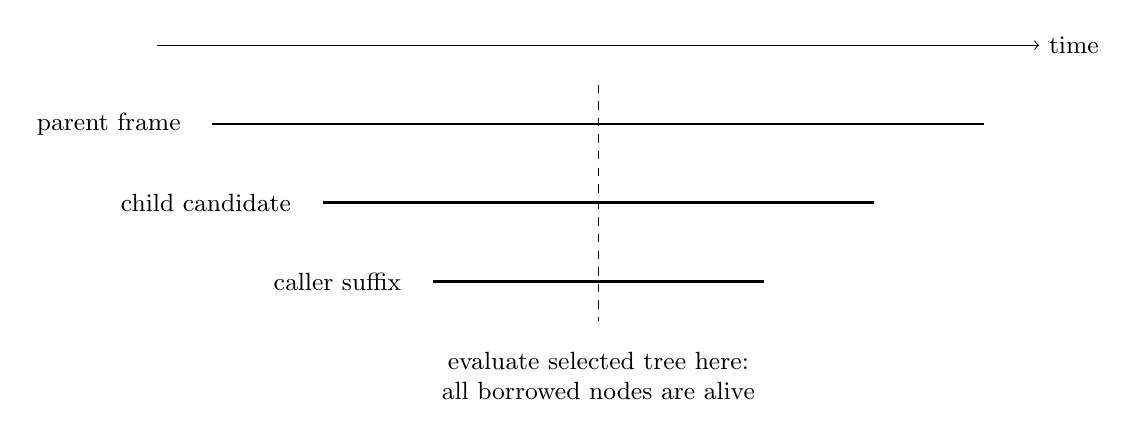
\begin{tikzpicture}[x=14mm,y=10mm]
\draw[->] (0,0)--(8,0) node[right,font=\small] {time};
\draw[line width=1pt] (0.5,-1)--(7.5,-1);
\draw[line width=1pt] (1.5,-2)--(6.5,-2);
\draw[line width=1pt] (2.5,-3)--(5.5,-3);
\draw[dashed] (4,-0.5)--(4,-3.5);
\node[anchor=east,font=\small] at (0.3,-1) {parent frame};
\node[anchor=east,font=\small] at (1.3,-2) {child candidate};
\node[anchor=east,font=\small] at (2.3,-3) {caller suffix};
\node[font=\small,align=center] at (4,-4.2) {evaluate selected tree here:\\all borrowed nodes are alive};
\end{tikzpicture}
\caption{Synchronous continuation calls preserve candidate lifetimes through commitment; no candidate pointer escapes the search stack.}
\label{fig:ch52-lifetime}
\end{figure}

The terminal engine simulates an epsilon NFA and remembers its longest accepted prefix.
It uses byte offsets and explicit input length, so a zero byte inside the buffer is data rather than an end marker.
Semantic terminal values are copied and nul-terminated for convenient C actions; actions that inspect binary data must use the supplied length rather than \code{strlen}.
Layout matching is repeated until no positive-length match remains.
The skip regex is not rewritten to a broader whitespace class: a request to skip spaces and tabs must not unexpectedly skip newlines.

\section{Specify failure, ownership, and budgets}
\label{sec:ch52-api}

The entry point accepts a source pointer, its byte length, and an optional \code{AULimits} pointer.
It returns \code{AUResult}, containing status, semantic value, furthest diagnostic offset, one expected spelling, search-step count, and an allocation list.
Table~\ref{tab:ch52-status} records which conclusions each status permits.
An empty production can succeed with a null value, so success is never tested by the value pointer alone.

\begin{table}[htbp]
\caption{Status, not the semantic pointer, determines whether recognition established a result.}
\label{tab:ch52-status}
\centering
\begin{tabular}{lp{0.72\linewidth}}
\toprule
Status & Meaning \\
\midrule
\code{AU\_OK} & Complete derivation selected and actions evaluated; value may be null. \\
\code{AU\_SYNTAX} & All permitted alternatives exhausted without complete recognition. \\
\code{AU\_LIMIT} & Search or native-recursion budget exhausted; membership undecided. \\
\code{AU\_NOMEM} & Committed-tree evaluation could not allocate required storage. \\
\code{AU\_INVALID} & Invalid API arguments, such as null input or unsupported depth limit. \\
\bottomrule
\end{tabular}
\end{table}

\code{au\_alloc} adds storage to the returned result's allocation list.
User constructors must check its return before writing and return without further work when allocation fails.
\code{au\_result\_free} releases those blocks and clears the value pointer; callers invoke it on every result, including failures.
Actions that allocate with an unrelated allocator retain their own ownership obligations.
There is no attempt to reverse arbitrary external effects if a later committed action fails: deferral prevents effects from rejected syntax branches, not transactions across all user code.

The default budget is one million charged search/NFA rounds and depth $256$.
The depth is an engine-frame count, not a language nesting depth; one source construct can require several pending continuation frames.
The hard maximum is $256$, and a zero budget deliberately returns a resource limit.
Each NFA round can inspect up to its number of states, so a step budget is not a literal CPU-instruction bound.
User actions are outside this search budget and must terminate under their own contract.

Diagnostics retain the furthest terminal-start or end-check offset reached by a failed attempt.
On a tie, the first expected spelling is retained.
The result is a reproducible explanation of failed search, not a claim that the deepest speculative path is always the best human explanation.
Recovery, merged expected-token sets, and context-ranked diagnostics are possible extensions.
They are not silently implemented by saving a cursor alone.

\section{Build, execute, and test the generated program}
\label{sec:ch52-tests}

The arithmetic example lives in \path{example-code/aurocks/calculator.g}.
It uses separate sum, product, and atom rules, plus nullable tails, and evaluates \code{2+3*(4+1)} to $17$.
Its driver accepts at most nine one-digit leaves, keeping the largest possible positive product below the minimum C99 \code{LONG\_MAX}.
This is an explicit demonstration domain; a general calculator must implement checked or arbitrary-precision arithmetic.

\begin{verbatim}
perl support/aurocks.pl example-code/aurocks/calculator.g > /tmp/opencode/calc.c
cc -std=c99 /tmp/opencode/calc.c -o /tmp/opencode/calc
/tmp/opencode/calc '2+3*(4+1)'
\end{verbatim}

Algorithm~\ref{alg:ch52-consume} summarizes the embedding contract.
The returned value is valid only while its owning result remains alive.
For long-lived compiler ASTs, the application can transfer data into its own compilation arena or arrange that arena's lifetime explicitly.

\begin{algorithm}[htbp]
\caption{Consume a generated parser result without confusing failure categories.}
\label{alg:ch52-consume}
\begin{pseudocode}
\Require generated parser, source buffer, explicit resource policy
\Ensure result storage released and only successful values consumed
\State $r\gets\Call{Parse}{buffer,length,limits}$
\If{$r.status=OK$}
  \State consume or copy $r.value$, permitting a null semantic value
\ElsIf{$r.status=SYNTAX$}
  \State report failed recognition at the recorded byte offset
\Else
  \State report the resource or API failure separately
\EndIf
\State release all result-owned allocations
\end{pseudocode}
\end{algorithm}

The end-to-end tests invoke the real Perl generator, compile the emitted C with strict warnings, and execute it under GCC and Clang, both normally and with address/undefined-behavior sanitizers.
They compare the recursive grammar $S\to aSb\mid\epsilon$ against an independent recognizer for $a^n b^n$ on all $511$ words over $\{a,b\}$ of length at most eight.
For accepted words, the recorded exact work budget succeeds, while one fewer charged step returns \code{AU\_LIMIT}.
Other tests exercise nullable-prefix recursion rejection, malformed grammar tokens, action references, nested action braces, regex bounds, character classes, embedded zero bytes, complete-input checks, and forced allocation failure.

The backtracking regression checks effects as well as membership: \code{ab} and \code{abb} each run exactly two selected production actions; \code{abx} runs none.
Another test deliberately checks that \code{/a+/ 'a'} rejects \code{aa}, preserving the documented atomic terminal policy.
These negative tests prevent an apparently helpful change from silently altering the language.
The suite is run with
\begin{verbatim}
PYTHONDONTWRITEBYTECODE=1 python3 -m unittest discover \
  -s support -p test_aurocks.py -v
\end{verbatim}
Python is test-driver tooling; the generator is Perl and the generated runtime is C99.
The finite tests complement the invariants of the earlier chapters rather than proving correctness for every grammar and input.

\section{Exercises}
\label{sec:ch52-exercises}
\begin{enumerate}
\item\label{ex:ch52-cycle} Draw the nullable-prefix graph for $S\to AB$, $A\to\epsilon$, $B\to S\mid b$ and identify the cycle that must be rejected.
\item\label{ex:ch52-null} Write an epsilon action returning a null value. State the status and ownership checks required from its caller.
\item\label{ex:ch52-atomic} Rewrite $S\to/a^+/\ a$ using recursive grammar alternatives over literal \code{a} so that \code{aa} is accepted under the case-study lexical policy.
\item\label{ex:ch52-effects} Explain why deferring actions prevents a failed parse from printing speculative output, but does not make several committed actions an atomic transaction under allocation failure.
\end{enumerate}
Worked answers are included with the examples.

\section{Further reading}
\label{sec:ch52-reading}
Grune and Jacobs give the broader parsing-method context for the implementation and its deliberate restrictions~\cite{grune-2008-parsing}.
Hopcroft, Motwani, and Ullman justify the automata machinery used for terminal recognition~\cite{hopcroft-2007-automata}.
The GLL combinator work shows how shared descriptors and returns extend top-down parsing beyond this depth-first native-stack design~\cite{vanbinsbergen-2018-gll}.
